\documentclass[11pt]{article}

\usepackage[margin=1.1in]{geometry}
\usepackage{amsmath}
\usepackage{amssymb}
\usepackage{amsthm}
\usepackage{mathrsfs}
\usepackage{booktabs}
\usepackage{enumitem}
\usepackage{tikz}
\usepackage[hidelinks]{hyperref}

\theoremstyle{plain}
\newtheorem{theorem}{Theorem}[section]
\newtheorem{proposition}[theorem]{Proposition}
\newtheorem{lemma}[theorem]{Lemma}
\newtheorem{corollary}[theorem]{Corollary}
\newtheorem{conjecture}[theorem]{Conjecture}
\theoremstyle{definition}
\newtheorem{definition}[theorem]{Definition}
\newtheorem{example}[theorem]{Example}
\theoremstyle{remark}
\newtheorem{remark}[theorem]{Remark}

% ---- source calculus, following the companion note ----
\newcommand{\quo}[1]{@#1}
\newcommand{\drp}[1]{{*}#1}
\newcommand{\inp}[3]{\mathsf{for}(\,#1 \leftarrow #2\,)#3}
\newcommand{\out}[2]{#1!(#2)}
\newcommand{\nil}{\mathbf{0}}
\newcommand{\enc}[1]{[\![#1]\!]}
\newcommand{\nequiv}{\equiv_{\mathcal{N}}}
\newcommand{\Ctx}{\mathscr{C}}
\newcommand{\Obs}{\mathcal{D}}
\newcommand{\bisim}{\approx}
\newcommand{\fn}{\mathrm{fn}}
\newcommand{\nms}[1]{\mathcal{N}^{*}(#1)}
\providecommand{\xLongrightarrow}[1]{\mathrel{\overset{#1}{\Longrightarrow}}}

% ---- combinators ----
\newcommand{\mm}{\mathsf{m}}
\newcommand{\dd}{\mathsf{d}}
\newcommand{\kk}{\mathsf{k}}
\newcommand{\fw}{\mathsf{fw}}
\newcommand{\bl}{\mathsf{b}_{\mathsf{l}}}
\newcommand{\br}{\mathsf{b}_{\mathsf{r}}}
\newcommand{\sy}{\mathsf{s}}
\newcommand{\ev}{\mathsf{e}}
\newcommand{\qq}{\mathsf{q}}
\newcommand{\Wt}{\mathsf{W}}
\newcommand{\cons}{\mathsf{cons}}
\newcommand{\red}{\longrightarrow}
\newcommand{\wred}{\longrightarrow^{*}}
\newcommand{\scong}{\equiv}

\title{\textbf{Name-Free Combinators for the Rho Calculus}\\[4pt]
\large A repair, a linear encoding, and the one operation that was missing}
\author{F1R3FLY.io research note}
\date{September 2026 --- draft 3 (rewritten), revision 1, 22 September 2026}

\begin{document}
\maketitle

\begin{abstract}
\noindent
The name-free concurrent combinators of \emph{Name-free combinators for
concurrency} were proposed as a target into which the rho calculus embeds
with no binders at all. This note asks whether the embedding is correct. It
is not, and the repairs are instructive.

The published calculus is unsound, and the defect is the conflation of the
rho calculus drop with the guard that consumes a message and runs its
payload: under $\drp{\quo{P}} = P$ that conflation makes every running
process a redex. Separating the two constructors repairs it and leaves two
sound presentations, both given here as operational theories --- one keeping
the equation and decoding by it, one omitting it, sorting message payloads as
processes, and decoding by the $\ev$ rule, which is then literally the drop
clause of Meredith--Radestock substitution promoted from the metatheory.
Neither can be assembled piecemeal from the other, and only the second lets a
decoder return an optimised representative rather than an equal one, which is
what an implementation that normalises on decode actually does.

Repaired, the combinators still fall short of the rho calculus by exactly one
capability: they have a name destructor and no name constructor, so they can
open a name that arrives at runtime but never build one. A name-closure lemma
makes this the bottom edge of an expressiveness lattice over subsets of the
atoms, developed here in place of a single separation theorem. The lattice
carries two orderings, expressive and observational, which do not coincide,
because the calculus has no name hiding; both are drawn. Four constructors
close the gap, one for each node a rebuilt name can have, and the translation
then covers the whole calculus with no fragment restriction.

Reflection also buys an unexpected efficiency. A continuation can be quoted
and released by a three-atom gate rather than rewritten atom by atom, so
prefix elimination is linear where Yoshida's is $\Theta(3^{d})$ in the
nesting depth of inputs. Correctness is established as full abstraction
relative to encoded contexts, in the sense of the companion note, and the
restriction to encoded observers is shown to be forced --- which is also
where the storage combinator earns its place, since it holds a continuation
invisibly rather than as an observable message. A final section gives an
alternative presentation in which the message and the store are not primitive
but the nullary members of the constructor family, leaving a calculus of
routers, one destructor, and constructors.

\paragraph{Revision 1.} Lemma~\ref{lem:atomcount} was stated for the plain
count of non-message atoms, which $\bl$, $\br$ and $\sy$ do not decrease: each
consumes itself and produces a $\fw$. The term
$\bl(a,b) \mid \mm(a,v) \mid \mm(v,x)$ has one non-message atom and reduces in
two steps, so the length bound of Proposition~\ref{prop:sn} failed with it.
Both are restated here for a weighted count that every rule but $\ev$'s does
decrease; strong normalisation, the strictness of the destructor edge, and
every other result of the note are unchanged. Numbering is preserved.
\end{abstract}

\tableofcontents

\section{Introduction}
\label{sec:intro}

The rho calculus\footnote{The name is an acronym and a pun. It abbreviates the
\textbf{r}eflective \textbf{h}igher \textbf{o}rder calculus; dropping the
periods from r.h.o.\ gives the English transliteration of the Greek letter
following $\pi$, marking the calculus as successor to the $\pi$-calculus. It
is written ``rho calculus'', never with the Greek letter.} has no
name-restriction operator: names are quoted processes, and freshness is
obtained by quotation rather than by a binder. It nonetheless has a binder,
the input prefix. Yoshida showed how to eliminate the input binder of the
asynchronous $\pi$-calculus in favour of combinators, at the cost of keeping
$\mathsf{new}$. The combination is suggestive: a calculus with no
$\mathsf{new}$, compiled by a discipline that removes the remaining binder,
should give a concurrency calculus with no bound names whatsoever. That is
what \cite{rhocomb} proposed. This note asks whether the proposal works.

\paragraph{Findings.}

\begin{enumerate}[leftmargin=1.6em]

\item \textbf{One equation breaks the calculus.} The published combinators
inherit $\drp{\quo{P}} \scong P$ from a presentation in which quote and drop
are mutually inverse up to structural congruence. In the combinator setting
the drop is not a process former but a guard, and since every name is
$\quo{Q}$ for some $Q$, the identification makes an arbitrary running process
match the guard. Proposition~\ref{prop:defect}: for all $P,Q$,
$Q \mid \mm(\quo{Q},\quo{P}) \red P$. The repair is to separate the drop from
the guard, which leaves the equation optional;
\S\ref{sec:two} gives both presentations and \S\ref{sec:why} compares
them.

\item \textbf{Reflection was half-implemented.} The rule
$\ev(a) \mid \mm(a,\quo{P}) \red P$ opens a name that arrives at runtime.
Nothing builds one. Lemma~\ref{lem:nonames}: combinator reduction never
produces a name that was not already present in the redex, hereditarily.
Rho reduction does, at every step, because substituting under a quotation
turns $\quo{(\drp{y} \mid R)}$ into $\quo{(Q \mid R)}$ --- a name in neither
participant. Lemma~\ref{lem:nonames} is the bottom edge of the lattice of
\S\ref{sec:lattice}: no combinator term of the published calculus is
equivalent to $\inp{y}{a}{\out{\quo{(\drp{y} \mid \drp{y})}}{\nil}}$. The
lattice has two orderings, expressive and observational, which do not
coincide, because the calculus has no name hiding.

\item \textbf{Four constructors close the gap.} The missing operation is
the construction of a name from names. It is supplied by constructors of the
shape $\cons_{\mid}(a,b,c) \mid \mm(a,\quo{P}) \mid \mm(b,\quo{Q}) \red
\mm(c,\quo{(P \mid Q)})$, one for each node a rebuilt name can have.
Proposition~\ref{prop:four} shows four are enough for the whole rho calculus:
parallel composition, message, and the two atoms that can head a translated
input. There is no name-opaque fragment to restrict to.

\item \textbf{The storage combinator is about opacity, not power.}
$\qq(a,P)$, released by a forwarder rather than by a message, satisfies the
no-name-creation lemma and so adds nothing to expressiveness. What it adds is
silence: it is a message that only a redirection can read, which is what
stored code and intermediate results of name construction need if the
encoding is to be opaque to observers (\S\ref{sec:q},
Remark~\ref{rem:loudquiet}).

\item \textbf{Prefix elimination is linear.} Reflection allows a continuation
to be quoted once and released by a three-atom gate. Yoshida must instead
push the prefix through the body, splitting at every parallel composition and
delaying every atom, which costs a constant factor per level of nesting:
Proposition~\ref{prop:blowup} computes $(3^{d-1}+1)/2$ atoms on an explicit
family where the reflective encoding gives $3d+1$.

\item \textbf{Correctness is full abstraction relative to encoded contexts.}
Following \cite{nowns}, observation is by context-labelled bisimilarity with
the observer class taken to be the image of the translation on source
contexts. Theorem~\ref{thm:fullabs}; and Proposition~\ref{prop:forced}, that
the restriction is forced rather than convenient, by the same argument that
forces it there.

\end{enumerate}

\S\ref{sec:altpres} gives the alternative presentation in which $\mm$ and
$\qq$ are the nullary constructors. \S\ref{sec:corrigenda} lists the
corrigenda to \cite{rhocomb}.

\paragraph{Notation.} \cite{rhocomb} writes $\mathsf{*}$ for three distinct
things: Yoshida's replication, the rho calculus drop, and the combinator that
consumes a message and runs its payload. We write $\ev$ for the last and
reserve $\drp{x}$ for the drop. The distinction between the second and the
third is one of the points of \S\ref{sec:why}.

\section{The rho calculus}
\label{sec:rho}

We follow \cite{MeredithRadestock05}.

\begin{definition}[Syntax]
\begin{align*}
  P,Q &\;::=\; \nil \;\mid\; \inp{y}{x}{P} \;\mid\; \out{x}{P}
        \;\mid\; \drp{x} \;\mid\; P \mid Q\\
  x,y &\;::=\; \quo{P}
\end{align*}
\end{definition}

$\fn(P)$ is as usual, with $\fn(\inp{y}{x}{P}) = \{x\} \cup (\fn(P)\setminus
\{y\})$. $\nms{P}$ is the set of names occurring anywhere in $P$, including
hereditarily inside quotations.

\begin{definition}[Structural congruence, name equivalence]
$\scong$ is the least congruence containing $\alpha$-equivalence and making
$(\mathsf{Proc},\mid,\nil)$ an abelian monoid. $\nequiv$ is the least
congruence on names with $\quo{\drp{x}} \nequiv x$, and $\quo{P} \nequiv
\quo{Q}$ whenever $P \scong Q$.
\end{definition}

The converse identification $\drp{\quo{P}} \scong P$ is deliberately absent.
Its work is done by substitution.

\begin{definition}[Semantic substitution]
\label{def:subst}
On names, $y\{\quo{Q}/y\} = \quo{Q}$ and $\quo{P}\{\quo{Q}/y\} =
\quo{(P\{\quo{Q}/y\})}$. On processes, the structural clauses together with
\[
  (\drp{y})\{\quo{Q}/y\} \;=\; Q,
  \qquad
  (\drp{z})\{\quo{Q}/y\} \;=\; \drp{z}\quad (z \neq y).
\]
\end{definition}

The drop clause is the whole of the difference between semantic and syntactic
substitution. Syntactic substitution returns $\drp{\quo{Q}}$, and one then
needs $\drp{\quo{Q}} \scong Q$ to recover the meaning. Semantic substitution
decodes at the moment of substitution and returns a process bisimilar to any
other faithful decoding rather than congruent to a canonical one; the decoder
is free to return an optimised representative.

\begin{definition}[Reduction]
\[
  \frac{x_{t} \nequiv x_{s}}
       {\inp{y}{x_{t}}{P} \mid \out{x_{s}}{Q} \red P\{\quo{Q}/y\}}
  \qquad
  \frac{P \red P'}{P \mid Q \red P' \mid Q}
  \qquad
  \frac{P \scong P' \ \ P' \red Q' \ \ Q' \scong Q}{P \red Q}
\]
\end{definition}

\begin{definition}
$P$ is \emph{guarded-drop} if every $\drp{x}$ in $P$ has $x$ a variable bound
by an enclosing input.
\end{definition}

\begin{lemma}
\label{lem:guarded}
Guarded-drop is preserved by reduction, and no subterm $\drp{\quo{Q}}$ ever
arises from a guarded-drop term.
\end{lemma}

\begin{proof}
A drop can acquire a ground name only by substitution, and
Definition~\ref{def:subst} eliminates the drop rather than instantiating it.
Every other clause is structural.
\end{proof}

A term $\drp{\quo{Q}}$ may still be written by hand, and is then inert. For
such terms $\drp{\quo{Q}}$ and $Q$ are related by the decoding bisimulation
rather than by $\scong$, which is the latitude the original presentation was
designed to leave. Source terms are assumed guarded-drop throughout.

\section{The rho combinators}
\label{sec:comb}

\subsection{Notation}

We present the combinators as an operational theory: formation judgements,
equations, and named rewrite rules, each under a context assigning sorts to
its variables. There are two sorts, $\mathsf{N}$ for names and $\mathsf{P}$
for processes. This is heavier than the grammar of \cite{rhocomb} and earns
its weight in \S\ref{sec:two}, where two presentations differ precisely in
which sort a message payload has, a distinction a single-sorted grammar hides.

\subsection{Formation}

\[
\begin{array}{l@{\qquad}l}
 a,b : \mathsf{N} \vdash \mm(a,b) : \mathsf{P}
   & a,b : \mathsf{N} \vdash \bl(a,b) : \mathsf{P}\\
 a,b,c : \mathsf{N} \vdash \dd(a,b,c) : \mathsf{P}
   & a,b : \mathsf{N} \vdash \br(a,b) : \mathsf{P}\\
 a : \mathsf{N} \vdash \kk(a) : \mathsf{P}
   & a,b,c : \mathsf{N} \vdash \sy(a,b,c) : \mathsf{P}\\
 a,b : \mathsf{N} \vdash \fw(a,b) : \mathsf{P}
   & a : \mathsf{N} \vdash \ev(a) : \mathsf{P}\\
 a : \mathsf{N},\ p : \mathsf{P} \vdash \qq(a,p) : \mathsf{P}
   & a,b,c : \mathsf{N} \vdash \cons(a,b,c) : \mathsf{P}\\
 a,b,c : \mathsf{N} \vdash \cons_{\mm}(a,b,c) : \mathsf{P}
   & a,b,c,f : \mathsf{N} \vdash \cons_{\dd}(a,b,c,f) : \mathsf{P}\\
 a,b,c,f : \mathsf{N} \vdash \cons_{\sy}(a,b,c,f) : \mathsf{P}
   & \vdash \nil : \mathsf{P}\\
 p,q : \mathsf{P} \vdash p \mid q : \mathsf{P}
   & p : \mathsf{P} \vdash \quo{p} : \mathsf{N}\\
 a : \mathsf{N} \vdash \drp{a} : \mathsf{P}\\
\end{array}
\]

We write $\cons$ for the parallel constructor, $\cons_{\mid}$ where the
subscript aids reading. Note that $\drp{-}$ and $\ev$ are distinct
constructors: the first is the drop of the rho calculus, the second the guard
that consumes a message and runs its payload. Conflating them is the defect
of \S\ref{sec:defect}.

\subsection{Equations, and the two presentations}
\label{sec:two}

\begin{definition}[Equations]
\label{def:combcong}
Common to both presentations:
\[
\begin{array}{l}
 p,q : \mathsf{P} \vdash p \mid q = q \mid p\\
 p,q,r : \mathsf{P} \vdash (p \mid q) \mid r = p \mid (q \mid r)\\
 p : \mathsf{P} \vdash p \mid \nil = p\\
 a : \mathsf{N} \vdash \quo{\drp{a}} = a
\end{array}
\]
\end{definition}

The two presentations differ in one equation and, consequently, in the sort
of a message payload and in the form of the $\mathsf{eval}$ rule.

\paragraph{Presentation A (identified).} Add
\[
  p : \mathsf{P} \vdash \drp{\quo{p}} = p
\]
so that $\quo{-}$ and $\drp{-}$ are inverse bijections between the sorts.
Message payloads are names, $\mm(a,b)$ with $b : \mathsf{N}$, and decoding is
performed by the equation:
\[
  a,v : \mathsf{N} \vdash \mathsf{eval} : \ev(a) \mid \mm(a,v) \red \drp{v}
\]
which is the intended process because $\drp{\quo{p}} = p$.

\paragraph{Presentation B (original).} Omit that equation. Message payloads
are then processes, $\mm(a,p)$ with $p : \mathsf{P}$, matching the output
constructor $\out{x}{P}$ of the source calculus, and decoding is performed by
the rule:
\[
  a : \mathsf{N},\ p : \mathsf{P} \vdash \mathsf{eval} :
  \ev(a) \mid \mm(a,p) \red p
\]

\begin{remark}[The presentations are not interchangeable piecemeal]
\label{rem:notpiecemeal}
One cannot omit $\drp{\quo{p}} = p$ and keep name-sorted payloads. With
name-sorted payloads the only available rule is $\ev(a) \mid \mm(a,v) \red
\drp{v}$, and without the equation the result is a stuck drop; while
pattern-matching the payload as $\quo{p}$ is ambiguous, since
$\quo{\drp{a}} = a$ lets any $v$ be read as $\quo{\drp{v}}$, so the rule
could return either $\drp{v}$ or, when $v$ is literally $\quo{Q}$, the
process $Q$ --- and without the equation these differ. Sorting the payload as
a process removes the ambiguity, because the payload is then given rather
than recovered. The two presentations are thus each internally forced, and
the choice between them is the choice of where decoding happens.
\end{remark}

\begin{definition}[Rules]
\label{def:combred}
Common to both presentations, with the payload metavariable read as a name in
A and as a process in B:
\[
\begin{array}{l}
 a,b,c,v : \mathsf{N} \vdash \mathsf{dist} :
   \dd(a,b,c) \mid \mm(a,v) \red \mm(b,v) \mid \mm(c,v)\\
 a,v : \mathsf{N} \vdash \mathsf{kill} : \kk(a) \mid \mm(a,v) \red \nil\\
 a,b,v : \mathsf{N} \vdash \mathsf{forward} :
   \fw(a,b) \mid \mm(a,v) \red \mm(b,v)\\
 a,b,v : \mathsf{N} \vdash \mathsf{bind}_{\mathsf{l}} :
   \bl(a,b) \mid \mm(a,v) \red \fw(v,b)\\
 a,b,v : \mathsf{N} \vdash \mathsf{bind}_{\mathsf{r}} :
   \br(a,b) \mid \mm(a,v) \red \fw(b,v)\\
 a,b,c,v : \mathsf{N} \vdash \mathsf{synch} :
   \sy(a,b,c) \mid \mm(a,v) \red \fw(b,c)\\
 a,b : \mathsf{N},\ p : \mathsf{P} \vdash \mathsf{quote} :
   \fw(a,b) \mid \qq(a,p) \red \mm(b,\quo{p})\\
 a,b,c : \mathsf{N},\ p,r : \mathsf{P} \vdash \mathsf{make}_{\mid} :
   \cons(a,b,c) \mid \mm(a,\quo{p}) \mid \mm(b,\quo{r})
   \red \mm(c,\quo{(p \mid r)})\\
 a,b,c,u,v : \mathsf{N} \vdash \mathsf{make}_{\mm} :
   \cons_{\mm}(a,b,c) \mid \mm(a,u) \mid \mm(b,v)
   \red \mm(c,\quo{\mm(u,v)})\\
 a,b,c,f,u,v,w : \mathsf{N} \vdash \mathsf{make}_{\dd} :
   \cons_{\dd}(a,b,c,f) \mid \mm(a,u) \mid \mm(b,v) \mid \mm(c,w)
   \red \mm(f,\quo{\dd(u,v,w)})\\
 a,b,c,f,u,v,w : \mathsf{N} \vdash \mathsf{make}_{\sy} :
   \cons_{\sy}(a,b,c,f) \mid \mm(a,u) \mid \mm(b,v) \mid \mm(c,w)
   \red \mm(f,\quo{\sy(u,v,w)})
\end{array}
\]
together with the presentation's own $\mathsf{eval}$, closed under parallel
composition and under the equations, with subjects matched up to $\nequiv$.
\end{definition}

For the remainder we write payloads in presentation A's notation,
$\mm(a,\quo{p})$; under B read $\mm(a,p)$. No rule, lemma or proof below
distinguishes the two.

Reduction is nondeterministic and is meant to be. Two consumers may compete
for one message, as in $\dd(a,b,c) \mid \kk(a) \mid \mm(a,v)$; and two
producers may compete for one consumer, as in
$\fw(a,b) \mid \mm(a,v) \mid \qq(a,p)$, where $\fw$ is the consumer at $a$
and $\mm$ and $\qq$ both offer a value there. Neither is pathological and
neither is new: they are the two sides of the race the communication rule has
always had.

\begin{remark}[Departures from the published rules]
\label{rem:departures}
Three corrections are folded into Definition~\ref{def:combred} and are worth
flagging, since they are easy to reintroduce. The binders must produce
forwarders, $\br(a,b) \mid \mm(a,v) \red \fw(b,v)$ and
$\bl(a,b) \mid \mm(a,v) \red \fw(v,b)$; a version producing a message merely
duplicates $\mathsf{forward}$ and loses the only function these atoms have,
which is to bind the received name into a redirection --- the links of kinds
(o1) and (o2) in \S\ref{sec:translation} depend on it. $\fw$ is binary
throughout. And in the constructors the delivery channel $f$ must appear in
the atom's own argument list, distinct from the input channels.
\end{remark}

\subsection{The defect}
\label{sec:defect}

\begin{proposition}
\label{prop:defect}
Suppose $\drp{-}$ and $\ev$ are the same constructor, as in \cite{rhocomb},
where the guard is written $\mathsf{*}$; and suppose
$\drp{\quo{p}} = p$. Then for all $P,Q$,
\[
  Q \mid \mm(\quo{Q},\quo{P}) \;\red\; P.
\]
\end{proposition}

\begin{proof}
Every name is $\quo{Q}$ for some $Q$, so under the conflation
$\mathsf{*}(\quo{Q}) = Q$. Reduction is closed under the equations, so the
redex $\mathsf{*}(a) \mid \mm(a,\quo{P})$ with $a = \quo{Q}$ matches
$Q \mid \mm(\quo{Q},\quo{P})$, and the rule fires.
\end{proof}

An arbitrary running process can therefore be annihilated and replaced by an
arbitrary payload, by anyone who knows its quotation. No faithfulness theorem
survives this.

\begin{remark}
\label{rem:atom}
The hypothesis that does the damage is the conflation, not the equation. The
published grammar lists the guard under the process production alongside
parallel composition, which invites reading it as the drop; separating the
two constructors, as the formation rules above do, repairs the calculus and
leaves both presentations of \S\ref{sec:two} available. It is worth being
explicit that Proposition~\ref{prop:defect} is therefore not an argument
against $\drp{\quo{p}} = p$; the argument about that equation is in
\S\ref{sec:why}, and it is not an argument from soundness.
\end{remark}

\subsection{The storage combinator}
\label{sec:q}

\begin{remark}[$\qq$ is a message only a forwarder can read]
\label{rem:q}
The rule $\mathsf{quote}$ has the same right-hand side as
$\mathsf{forward}$. So $\qq(a,p)$ and $\mm(a,\quo{p})$ are indistinguishable
to a forwarder, and differ everywhere else: a message at $a$ may be consumed
by any of $\dd$, $\kk$, $\br$, $\bl$, $\sy$, $\ev$, a constructor or $\fw$,
whereas $\qq(a,p)$ may be consumed only by $\fw$. Since
$\fw(a,a) \mid \qq(a,p) \red \mm(a,\quo{p})$, $\qq$ is not a message awaiting
a trigger but the introduction form for a name constant, of which $\mm$ is
the already-manifest case.
\end{remark}

$\qq$ adds no expressive power --- it satisfies Lemma~\ref{lem:nonames} --- and
is not needed for the translation to be definable. What it provides is
opacity; see Remark~\ref{rem:loudquiet}.

\subsection{The name constructors}
\label{sec:cons}

Every rule but the last four moves names around or opens one. The last four
build one.

\begin{remark}
Each constructor takes names and returns a name: it assembles the quotation
of a single node from the quotations of its children, and the assembled name
is delivered as an ordinary message, so it may then be used as a subject, a
payload, or the input to a further constructor. Chaining them builds a name
of any shape from the outside in. The operation so performed is substitution
of a received name into a static term under a quotation, which is precisely
what the rho communication rule does and what \cite{rhocomb} has no
counterpart for.
\end{remark}

\begin{proposition}
\label{prop:four}
The four constructors of Definition~\ref{def:combred} suffice for the
translation of Definition~\ref{def:translation}: every name that must be
rebuilt at runtime is assembled by a chain of them.
\end{proposition}

\begin{proof}
A name to be rebuilt is $\quo{\enc{S}}$ for a source term $S$ with the bound
name free in it, and $\enc{-}$ is a homomorphism, so the nodes of
$\enc{S}$ are those of $S$. Take the path from an occurrence to the root;
every node off the path is static and is supplied as a constant message,
joined on by $\cons$. On the path, by
Definition~\ref{def:translation}: an occurrence under $\drp{-}$ is the
received name itself, needing no constructor; a parallel composition needs
$\cons$; an output $\out{v}{T}$ has image $\mm(\enc{v},
\quo{\enc{T}})$ and needs $\cons_{\mm}$, which covers both a dynamic
subject and a dynamic payload; and an input $\inp{z}{v}{T}$ has image
$D(\enc{v};\vec p) \mid G \mid \vec L$ in which $\enc{v}$ occurs only in
the head atom, which is $\dd(\enc{v},p_{0},q_{1})$ when $z$ occurs in $T$
and $\sy(\enc{v},b,c)$ when it does not; the remainder is static. Hence
$\cons_{\dd}$ and $\cons_{\sy}$. Duplication of the received name, when an
occurrence appears at several places, is supplied by $\dd$.
\end{proof}

\begin{remark}[The optimisations are not free]
\label{rem:optnotfree}
Proposition~\ref{prop:four} is stated for the general clauses. The
shortcuts of Remark~\ref{rem:opt} put a bound name into the argument of an
$\ev$ or a $\fw$, so a translation that takes them needs $\cons_{\ev}$ and
$\cons_{\fw}$ as well. Four is the count for the uniform translation, not a
lower bound over all translations.
\end{remark}

\begin{remark}[A more exotic alternative]
\label{rem:ctxindexed}
The family can be collapsed into one atom indexed by a static context:
$\cons[C](a,c) \mid \mm(a,v) \red \mm(c,\quo{C[v]})$ for a combinator
context $C$ with holes in name positions. This is derivable from the family
by the chain of Proposition~\ref{prop:four}, and conversely each member of
the family is the instance $C = A(-,\dots,-)$. It shortens the translation
and its proofs, at the price of an atom parameterised by a context rather
than by names --- a considerable conceptual cost, and one we do not think
worth paying in the presentation, though it is worth recording that the two
formulations have the same reach.
\end{remark}

\section{Where the decoding happens}
\label{sec:why}

Both presentations of \S\ref{sec:two} are sound, and every result in this
note holds under either. They differ in where the decoding of a name into
the process it quotes is performed, and that difference has consequences
worth stating rather than settling by fiat.

\paragraph{A puts the decoding in the equations.} $\drp{\quo{p}} = p$ makes
$\quo{-}$ and $\drp{-}$ inverse bijections, so $\mathsf{N} \cong \mathsf{P}$
and the two sorts carry the same information. Decoding is then not an event:
$\drp{v}$ \emph{is} the process, and $\mathsf{eval}$ need only produce the
term $\drp{v}$ and let the equation do the rest. The presentation is
economical and the rule is uniform in the payload.

\paragraph{B puts the decoding in the rule.} Without the equation, the
quotation of a process is an opaque name until some rule opens it, and
$\mathsf{eval}$ is that rule. This is the arrangement of
\cite{MeredithRadestock05}, where the corresponding clause is the drop case
of substitution, $(\drp{y})\{\quo{Q}/y\} = Q$. Compare it with the rule:
\[
  (\drp{y})\{\quo{Q}/y\} \;=\; Q
  \qquad\text{against}\qquad
  \ev(a) \mid \mm(a,p) \;\red\; p .
\]
These are the same equation, the first in the metatheory of a calculus with
substitution and the second in a calculus without one.

\paragraph{What B affords.} Because decoding is an event rather than an
identity, the decoder is free to return any process bisimilar to the one
quoted, rather than one equal to it. Under A that freedom is not available:
$\drp{\quo{p}}$ and $p$ are equal, so any two decodings of the same name are
equal, and a decoder that returns something else is not implementing the
equation.

This is not a hypothetical distinction. The F1R3FLY implementation normalises
on decode: what is handed back has been rearranged, and bound variables have
been replaced by de Bruijn indices. Neither transformation is derivable from
the equations of Definition~\ref{def:combcong}, which give only the monoid
laws and $\quo{\drp{a}} = a$. Under A the implementation is therefore not
sound for the stated theory; under B it is, because the theory only ever
claims the decoded process up to the equivalence of \S\ref{sec:clb}. An
implementation that normalises is evidence about which presentation is being
implemented, and it is B.

\paragraph{The surviving equation is load-bearing in both.}
$\quo{\drp{a}} = a$ is what makes it possible to send a name at all. A
message carries a process in B, so ``send the name $x$'' is
$\mm(v,\drp{x})$, whose quotation is $\quo{\drp{x}} = x$; in A the payload is
$x$ directly and the equation is what identifies the two readings. Every
name-forwarding clause of the translation depends on it.

\paragraph{A remark on sorts.} Under A the two sorts are isomorphic, so one
may ask what work the sorting does. It does the work of
Proposition~\ref{prop:defect}: an isomorphism is not an identification of
constructors, and keeping $\ev$ distinct from $\drp{-}$ is what prevents an
arbitrary process from matching a guard. The published single-sorted grammar
had no way to say this.

\section{Context-labelled bisimilarity}
\label{sec:clb}

We use the equivalence of the companion note \cite{nowns} rather than barbs,
for consistency with it. The two are close here --- both calculi are
name-passing, so barbs are an adequate observation --- but the context-labelled
form states the restriction on observers as part of the relation rather than
as a side condition on a set of names, and that restriction is the substance
of Theorem~\ref{thm:fullabs}.

\begin{definition}
\label{def:clb}
For a calculus with reduction $\red$ and contexts $\Ctx$, write
$P \xrightarrow{\,C\,} P'$ when $C[P] \red P'$ and
$P \xLongrightarrow{\,C\,} P'$ when $C[P] \wred P'$. For
$\Obs \subseteq \Ctx$, a symmetric $\mathcal{R}$ is an
\emph{$\Obs$-bisimulation} if $P \mathrel{\mathcal{R}} Q$ and
$P \xrightarrow{\,C\,} P'$ with $C \in \Obs$ imply
$Q \xLongrightarrow{\,C\,} Q'$ with $P' \mathrel{\mathcal{R}} Q'$. Write
$\bisim_{\Obs}$ for the largest such.
\end{definition}

On the source, $\Obs = \Ctx_{\mathrm{rho}}$, written $\bisim_{\mathrm{rho}}$.
On the target, $\Obs = \enc{\Ctx_{\mathrm{rho}}}$, the encodings of source
contexts. As in \cite{nowns} the labels are enabling contexts, not minimal
ones; minimality is the right long-run discipline and is developed in
\cite{BIHOL}, and nothing below needs it. Without it the label set is larger
and $\bisim_{\Obs}$ correspondingly finer, which makes completeness harder
rather than easier.

\section{The translation}
\label{sec:translation}

\subsection{Seeds}

The translation is indexed by a name, as the encoding of \cite{nowns} is
indexed by an address, so that it is compositional on the nose.

\begin{definition}
A \emph{seed} for $P$ is a name $s \notin \nms{P}$ modulo $\nequiv$. Set
$s^{\varepsilon} = s$, $s^{w0} = \quo{\mm(s^{w},\quo{\nil})}$ and
$s^{w1} = \quo{\kk(s^{w})}$ for a binary string $w$.
\end{definition}

\begin{lemma}
\label{lem:fresh}
$s := \quo{P}$ is a seed for $P$; and if $s$ is a seed for $P$ then the
$s^{w}$ are pairwise distinct modulo $\nequiv$ and none lies in $\nms{P}$.
\end{lemma}

\begin{proof}
Work with $\nequiv$-normal names, using that $\quo{\drp{x}} \to x$ is
terminating and confluent. Every name occurring in $P$ is the quotation of a
proper subterm, hence smaller than $\quo{P}$, so $\quo{P} \notin \nms{P}$.
The two constructors are injective on normal forms with disjoint images, so
$w \mapsto s^{w}$ is injective; and each $s^{w}$ mentions $s$ hereditarily.
\end{proof}

Names written $p_{i}$, $b$, $c_{i}$ below are $s^{w}$ for distinct $w$
allocated by position in the source term. Nothing depends on the particular
constructors.

\begin{remark}
\label{rem:namesize}
\cite{rhocomb} instead builds each constructed name by quoting the subterm it
must be fresh for, so every constructed name carries a copy of the body and
the output is quadratic in $|P|$ before any other cost is counted. Seeds give
names of size $|s| + O(|w|)$ with the same guarantee.
\end{remark}

\subsection{Gate and distributor}

\begin{definition}
For $b,c$ fresh, $G(p,S) := \sy(p,b,c) \mid \qq(b,S) \mid \ev(c)$; and
$D(x;p_{0}) := \nil$ with $p_{0} := x$, while for $k \geq 1$
\[
  D(x;p_{0},\dots,p_{k}) := \dd(x,p_{0},q_{1}) \mid \dd(q_{1},p_{1},q_{2})
  \mid \cdots \mid \dd(q_{k-1},p_{k-1},p_{k}).
\]
\end{definition}

\begin{lemma}
\label{lem:gate}
$G(p,S)$ has no reduction and is not a message. For any $v$,
\[
  G(p,S) \mid \mm(p,v) \red \fw(b,c) \mid \qq(b,S) \mid \ev(c)
  \red \mm(c,\quo{S}) \mid \ev(c) \red S,
\]
and these are the only reductions available. $D(x;p_{0},\dots,p_{k}) \mid
\mm(x,v) \wred \mm(p_{0},v) \mid \cdots \mid \mm(p_{k},v)$ in $k$ steps.
\end{lemma}

\begin{proof}
The three names $p,b,c$ are distinct, so no other pairing is possible, and
$\sy$ discards the payload. Before the forwarder is released there is no
$\fw$ at $b$, so $\qq(b,S)$ is inert by Remark~\ref{rem:q}. The claim for $D$
is immediate.
\end{proof}

The gate is the whole of the difference from Yoshida. It delays a
continuation of any size for three atoms and one quotation, because the
continuation travels as data.

\subsection{Clauses}

Occurrences of a bound name $y$ in a body $P$ fall into five kinds. Four are
occurrences at which $y$ is used as a name; the fifth is an occurrence inside
a quotation, at which a new name must be built.

\begin{table}[t]
\centering
\begin{tabular}{llll}
\toprule
 & occurrence of $y$ & in the quoted body & link\\
\midrule
(o1) & input subject $\inp{z}{y}{S}$ & subject $\to c_{i}$ & $\bl(p_{i},c_{i})$\\
(o2) & output subject $\out{y}{S}$ & subject $\to c_{i}$ & $\br(p_{i},c_{i})$\\
(o3) & forwarded name $\out{v}{\drp{y}}$ & atom deleted & $\fw(p_{i},\enc{v})$\\
(o4) & drop $\drp{y}$ in process position & $\to \ev(c_{i})$ & $\fw(p_{i},c_{i})$\\
(o5) & inside a quotation $\quo{S}$, $y \in \fn(S)$ & subject $\to c_{i}$
     & constructor chain for $S$\\
\bottomrule
\end{tabular}
\caption{Occurrence kinds. In (o5) the link is the chain of constructors of
Proposition~\ref{prop:four} that rebuilds $\quo{\enc{S}}$ from the received
name, delivering it at $c_{i}$, where the body uses it as it would any other
name. When several kinds coincide in one atom, the atom is deleted from the
body and the links are emitted together.}
\label{tab:links}
\end{table}

\begin{definition}[The translation]
\label{def:translation}
On names, $\enc{\quo{P}} := \quo{\enc{P}_{s^{w}}}$ where $w$ is the position
of that quotation in the enclosing term. On processes,
\[
\begin{array}{rcl}
  \enc{\nil}_{s} &=& \nil\\
  \enc{P \mid Q}_{s} &=& \enc{P}_{s^{0}} \mid \enc{Q}_{s^{1}}\\
  \enc{\out{x}{P}}_{s} &=& \mm(\enc{x}, \quo{\enc{P}_{s^{0}}})\\
  \enc{\inp{y}{x}{P}}_{s} &=& D(\enc{x};p_{0},\dots,p_{k}) \mid G(p_{0},B)
    \mid L_{1} \mid \cdots \mid L_{k}
\end{array}
\]
where $o_{1},\dots,o_{k}$ enumerate the free occurrences of $y$ in $P$, each
$o_{i}$ has a distinct proxy $c_{i}$, $L_{i}$ and the residue in $B$ are
given by Table~\ref{tab:links}, and $B$ is $\enc{P}_{s^{0}}$ with every
occurrence treated accordingly. $\enc{-}$ extends to contexts with the hole
expecting a seed; plugging is instantiation of the seed.
\end{definition}

The incoming message is duplicated $k+1$ times. One copy trips the gate,
which releases the continuation with each occurrence of the bound name
standing at a proxy. The other $k$ arrive at the links, each converting the
received name into the wiring its occurrence needs: $\br$ installs a
forwarder from the proxy to the received name, which is what an output
subject requires; $\bl$ installs one in the opposite direction, for an input
subject; $\fw$ delivers the name, for a forwarded name and for a drop, the
latter discharged by the $\ev$ in the body; and $\cons$ builds the name the
source would have built by substituting under the quotation.

\begin{remark}
\label{rem:opt}
Three special cases are cheaper and may be used directly:
$\enc{\inp{y}{x}{\nil}} = \kk(\enc{x})$,
$\enc{\inp{y}{x}{\drp{y}}} = \ev(\enc{x})$, and
$\enc{\inp{y}{x}{\out{v}{\drp{y}}}} = \fw(\enc{x},\enc{v})$ for $v \neq y$.
\end{remark}

\begin{example}
$P = \inp{y}{a}{\out{y}{\nil}}$ has one occurrence, of kind (o2), so
$\enc{P}_{s} = \dd(a,p_{0},p_{1}) \mid G(p_{0},\mm(c,\quo{\nil})) \mid
\br(p_{1},c)$. Supplying $\mm(a,\quo{\enc{R}})$ gives, in order,
$\mm(p_{0},\quo{\enc{R}}) \mid \mm(p_{1},\quo{\enc{R}})$; then
$\mm(c,\quo{\nil}) \mid \fw(c,\quo{\enc{R}})$; then
$\mm(\quo{\enc{R}},\quo{\nil}) = \enc{\out{\quo{R}}{\nil}}$.
\end{example}

\begin{example}[The witness]
\label{ex:witness}
$W = \inp{y}{a}{\out{\quo{(\drp{y} \mid \drp{y})}}{\nil}}$ has one
occurrence, of kind (o5): both drops resolve to the received name, and the
node above them is a parallel composition. So
\[
  \enc{W}_{s} = \dd(a,p_{0},p_{1}) \mid G(p_{0},\mm(c,\quo{\nil}))
  \mid \dd(p_{1},r_{1},r_{2}) \mid \cons_{\mid}(r_{1},r_{2},c),
\]
the inner duplicator supplying the received name to both arguments.
Receiving $\mm(a,\quo{\enc{R}})$ builds $\mm(c,\quo{(\enc{R}\mid\enc{R})})$,
and the released body sends $\nil$ on that name, which is
$\enc{\out{\quo{(R\mid R)}}{\nil}}$. Proposition~\ref{prop:consedges} shows
no term of the constructor-free calculus does this.
\end{example}

\section{Correctness}
\label{sec:correct}

\begin{lemma}[Compositionality]
\label{lem:compositional}
$\enc{C[P]} = \enc{C}[\enc{P}]$, on the nose.
\end{lemma}

\begin{proof}
Induction on $C$. Each clause of Definition~\ref{def:translation} mentions
its sub-translations only under a seed abstraction, and the hole occurs in
exactly one.
\end{proof}

\begin{lemma}[Linearity]
\label{lem:linearity}
In $\enc{P}_{s}$ every constructed name is the subject of at most one atom
and carries at most one message, and every atom participates in at most one
reduction.
\end{lemma}

\begin{proof}
Names are allocated by position, so distinct positions get distinct names by
Lemma~\ref{lem:fresh}; each clause emits each constructed name in one subject
position and at most one value position; every rule consumes both
participants. Copies arise only as payloads, and a payload carries its own
allocation.
\end{proof}

\begin{definition}[Link expansion]
$T' \succeq T$ if $T'$ is obtained from $T$ by replacing the subject $a$ of
finitely many atoms by distinct fresh proxies $c$ and adjoining $\fw(c,a)$
for a value-producing subject, $\fw(a,c)$ for a value-consuming one.
\end{definition}

\begin{lemma}
\label{lem:linkexp}
If $T' \succeq T$ and $T$ satisfies Lemma~\ref{lem:linearity} then
$T' \bisim_{\enc{\Ctx_{\mathrm{rho}}}} T$.
\end{lemma}

\begin{proof}
Relate $T'$ to $T$ when $T'$ is such an expansion with some adjoined
forwarders already discharged. A labelled step of $T$ through an expanded
atom is matched in $T'$ by the relay step followed by the same rule, giving
an expansion of the residue; a step of $T'$ is either a relay, matched by the
empty path, or an ordinary step matched directly. Linearity guarantees one
one-shot forwarder per occurrence suffices, the atom firing at most once. No
adjoined forwarder is a message, so no label distinguishes them.
\end{proof}

\begin{lemma}[Inertness]
\label{lem:inert}
$\enc{\inp{y}{x}{P}}_{s}$ has no reduction and contains no message.
\end{lemma}

\begin{proof}
The atoms present are the duplicators of $D$, the gate, and the links. None
is a message, and the atoms of $B$ are stored inside $\qq$, hence are not
subterms of any redex. No forwarder is present, so $\qq(b,B)$ is inert.
\end{proof}

\begin{lemma}[Name usage]
\label{lem:usage}
Let $y$ be bound in $\enc{P}_{s}$ by the translation of a rho input. Every
occurrence of the corresponding proxy is the subject of an atom of
$\enc{P}_{s}$ or an argument of a link. In particular an encoded context
neither names the constructed apparatus $s^{w}$ of a term it is composed
with, nor installs a forwarder at such a name.
\end{lemma}

\begin{proof}
Induction on $P$ using Definition~\ref{def:translation}: proxies are
introduced only by Table~\ref{tab:links} and used only there. For the second
claim, $\enc{C}$ allocates its constructed names from its own seed, and by
Lemma~\ref{lem:fresh} those are distinct from the seed powers of the term
plugged into the hole.
\end{proof}

\begin{lemma}[Release]
\label{lem:release}
$\enc{\inp{y}{x}{P}}_{s} \mid \mm(\enc{x},\quo{\enc{R}}) \wred T$ with
$T \bisim_{\enc{\Ctx_{\mathrm{rho}}}} \enc{P\{\quo{R}/y\}}_{s}$, in $k+3$
steps followed by at most $k$ administrative steps, and no other sequence is
available up to the order of independent steps.
\end{lemma}

\begin{proof}
By Lemma~\ref{lem:gate} the distributor delivers a copy to each $p_{i}$ and
the gate releases $B$. Each remaining copy meets its link. For (o1) and (o2)
the link yields a one-shot forwarder, which is the corresponding link
expansion; for (o3) it yields the message the translated output would have
been; for (o4) it yields $\mm(c_{i},\quo{\enc{R}})$, which with the $\ev(c_{i})$
in $B$ gives $\enc{R}$, and $(\drp{y})\{\quo{R}/y\} = R$ by
Definition~\ref{def:subst}, so the occurrence is discharged exactly; for (o5)
the chain of Proposition~\ref{prop:four} yields
$\mm(c_{i},\quo{\enc{S\{\quo{R}/y\}}})$, node by node, since $\enc{-}$ is a
homomorphism and each constructor reproduces one node of $\enc{S}$ with the
received name in place of the occurrence.
Hence $T \succeq \enc{P\{\quo{R}/y\}}_{s}$ and
Lemma~\ref{lem:linkexp} applies. Uniqueness follows from
Lemmas~\ref{lem:inert} and~\ref{lem:linearity}.
\end{proof}

The (o4) case is where the source's substitution and the target's $\ev$ rule
coincide: under presentation B both deliver $\enc{R}$ directly, and under A
both deliver $\drp{\quo{\enc{R}}}$, which the equation makes equal to it. The (o5) case is where the constructor earns its place.

\begin{lemma}[Seed independence]
\label{lem:seedind}
$\enc{P}_{s} \bisim_{\enc{\Ctx_{\mathrm{rho}}}} \enc{P}_{t}$ for seeds
$s,t$ of $P$.
\end{lemma}

\begin{proof}
Let $\beta_{s \to t}$ send $s^{w} \mapsto t^{w}$ and fix all other names; it
is a bijection by Lemma~\ref{lem:fresh} and extends to terms by metalevel
replacement, descending into quotations. It is not a rho substitution and no
combinator context performs it. Take $\mathcal{R} = \{(T,\beta_{s\to t}(T))\}$
for $T$ reachable from $\enc{P}_{s}$. A bijection on names preserves and
reflects $\nequiv$, hence the applicability of every rule of
Definition~\ref{def:combred}, including $\ev$ and $\cons$, whose right-hand
sides are computed from the redex and so commute with $\beta$. For the
labels, Lemma~\ref{lem:usage} shows an encoded context never names a seed
power of the term it observes, so no label distinguishes $T$ from its image.
\end{proof}

\begin{theorem}[Full abstraction relative to encoded contexts]
\label{thm:fullabs}
For all rho processes $P,Q$,
\[
  P \bisim_{\Ctx_{\mathrm{rho}}} Q
  \quad\Longleftrightarrow\quad
  \enc{P} \bisim_{\enc{\Ctx_{\mathrm{rho}}}} \enc{Q}.
\]
\end{theorem}

\begin{proof}
\emph{Forward.} Let $\mathcal{S}$ relate $T$ to $U$ whenever $T$ and $U$ are
reachable from $\enc{P'}$ and $\enc{Q'}$ respectively, for some
$P' \bisim Q'$, by the sequences of Lemma~\ref{lem:release}, modulo link
expansion and $\beta$. It is symmetric and contains
$(\enc{P},\enc{Q})$. Given a label $\enc{C}$, Lemma~\ref{lem:compositional}
gives $\enc{C}[\enc{P'}] = \enc{C[P']}$, so a target step from the plugged
term is, by Lemma~\ref{lem:inert}, either administrative --- matched by the
empty path, staying in $\mathcal{S}$ by
Lemmas~\ref{lem:linkexp} and~\ref{lem:seedind} --- or the first step of the
sequence of Lemma~\ref{lem:release}, in which case $C[P'] \red P''$ in the
source and the matching source step for $Q'$ transfers back along the same
lemma.

\emph{Backward.} A source step $C[P] \red P''$ is, by
Lemma~\ref{lem:release} read left to right, matched by
$\enc{C}[\enc{P}] \wred T \bisim \enc{P''}$; so a distinguishing source
context yields a distinguishing encoded context, and the contrapositive is
the claim.
\end{proof}

\begin{proposition}[The restriction is forced]
\label{prop:forced}
There are rho processes $P \bisim_{\Ctx_{\mathrm{rho}}} Q$ and a combinator
context $C \notin \enc{\Ctx_{\mathrm{rho}}}$ with
$C[\enc{P}] \not\bisim C[\enc{Q}]$.
\end{proposition}

\begin{proof}
The seed is computed by the translation from the source, so an arbitrary
combinator context can name $s^{w}$; take $C = [\,\cdot\,] \mid \fw(b,u)$ for
the gate name $b$ of a translated input and an observable $u$. By
Lemma~\ref{lem:gate} this extracts the stored continuation at $u$,
distinguishing two source terms that differ only in a continuation not
otherwise reachable. By Lemma~\ref{lem:usage} no encoded context installs
such a forwarder.
\end{proof}

\begin{remark}
This is the same shape as the corresponding result in \cite{nowns}, and for
the same underlying reason: the target manufactures names the source does not
have, and an unrestricted observer of the target may use them. There the
names are addresses; here they are seed powers. In neither case is the
restriction a weakening of the theorem --- it is the theorem's shape. Note
also that $\qq$ is doing real work in Proposition~\ref{prop:forced}: with the
continuation stored as $\mm(b,\quo{B})$ the context would not even need to
act, since the store would be a message and hence directly observable.
\end{remark}

\begin{remark}[Loud and quiet]
\label{rem:loudquiet}
With the constructors in the calculus the point generalises. A construction chain
parks each intermediate result as a message on a constructed name, so the
whole dataflow of name-building is observable to an unrestricted context, and
Table~\ref{tab:links} (o5) makes such chains common. The question $\qq$
answers for the nullary case --- should a stored value be loud or quiet? ---
therefore applies at every arity, and a uniform treatment would give each
constructor a quiet variant emitting $\qq(c,\cdot)$ rather than
$\mm(c,\cdot)$. We have not done this, and it is the main design question
left open by \S\ref{sec:altpres}.
\end{remark}

\section{Complexity of the target term}
\label{sec:complexity}

Let $|P|$ count atoms and $d(P)$ the nesting depth of input prefixes.

\begin{proposition}
\label{prop:linear}
$|\enc{P}_{s}| = O(|P|)$, and the textual size is
$O(|P|\cdot(|s| + \log|P|))$.
\end{proposition}

\begin{proof}
The clauses for $\nil$, parallel composition and output add at most one atom
each. An input adds $k$ duplicators, three gate atoms and $k$ links, where
$k$ counts occurrences of the bound name; the body is translated once and
appears once, inside a quotation. Summing $k$ over binders counts each
occurrence once. A link of kind (o5) is a chain of $O(|S|)$
constructors by Proposition~\ref{prop:four}, which is within the same bound
since $S$ is a subterm. Textual size follows from $|s^{w}| = |s| + O(|w|)$ with $O(|P|)$
names allocated.
\end{proof}

Yoshida must distribute the prefix through the body: her rule (I) splits at
every parallel composition, inserting a duplicator, and her rules (V) and
(VI) delay every atom behind its own synchroniser. Each prefix therefore
multiplies the body.

\begin{proposition}
\label{prop:blowup}
Let $P_{d} = \inp{x_{1}}{a}{\inp{x_{2}}{a}{\cdots \inp{x_{d}}{a}{\nil}}}$, so
$|P_{d}| = d+1$ and $d(P_{d}) = d$. Yoshida's elimination yields
$T(d) = (3^{d-1}+1)/2$ atoms, where $T(1) = 1$ and $T(j+1) = 3T(j)-1$, while
$|\enc{P_{d}}| = 3d+1$.
\end{proposition}

\begin{proof}
The innermost prefix gives one atom by her rule (III). If the body of the
next prefix has $n$ atoms, none mentioning the bound name, rule (I) inserts
$n-1$ duplicators along a binary tree and rule (VI) replaces each atom by a
synchroniser and a relabelled copy, giving $2n + (n-1)$. No other rule
applies, so the count is exact. For the reflective encoding each prefix has
no occurrences, contributing an empty distributor and one gate.
\end{proof}

\begin{corollary}
Prefix elimination with reflection is exponentially more succinct than
without it, in the nesting depth of inputs.
\end{corollary}

\begin{remark}
The mechanism is that Yoshida cannot store a continuation, so ``wait, then
behave like $T$'' must be implemented by rewriting $T$ itself, and a
constant-factor expansion composes multiplicatively down a nesting chain.
Reflection stores $T$ as the name $\quo{T}$ and pays only for the gate. We do
not claim $3^{d}$ is optimal for her calculus, only that it is what her rules
give; an unconditional lower bound would be a statement about all encodings.
\end{remark}

\section{An expressiveness lattice}
\label{sec:lattice}

Yoshida's separation results are not a single theorem but a lattice: subsets
of the combinators ordered by inclusion, with each strict edge witnessed by a
behaviour the smaller set cannot produce. This section sets up the
corresponding lattice for the rho combinators. It has a feature hers does
not, which is visible from the start and is a consequence of having no name
hiding: some edges are strict against arbitrary observers and collapse
against encoded ones, so what we have is not one lattice but a family indexed
by the observer class of Definition~\ref{def:clb}.

Throughout, $\mm$ is not a candidate for removal: it is the medium, and a
calculus without it has no communication to analyse. The candidates are the
six routers $\dd,\kk,\fw,\bl,\br,\sy$, the destructor $\ev$, the store $\qq$,
and the four constructors.

\subsection{Three invariants}

Each proved edge below comes from an invariant preserved by every rule of the
smaller set and violated by a witness in the larger.

\begin{lemma}[Name closure]
\label{lem:nonames}
Let $S$ be a set of constructors and $T$ a term over $S$. Every name
occurring in a reduct of $T$ lies in the closure of $\nms{T}$ under the node
shapes $\{A : \cons_{A} \in S\}$, modulo $\nequiv$.
\end{lemma}

\begin{proof}
Induction on reduction. Every rule other than the constructor rules has, on
its right, only names occurring on its left: for
$\ev(a) \mid \mm(a,\quo{P}) \red P$ the names of $P$ are hereditarily among
those of $\quo{P}$, and for $\fw(a,b) \mid \qq(a,P) \red \mm(b,\quo{P})$ both
$b$ and $\quo{P}$ occur in the redex. A constructor rule for shape $A$ emits
$\mm(c,\quo{A(v_{1},\dots,v_{n})})$, whose name is $A$ applied to names
already present. Structural congruence introduces no names.
\end{proof}

\begin{lemma}[Atom count]
\label{lem:atomcount}
Weight atoms by $\Wt(\bl) = \Wt(\br) = \Wt(\sy) = 2$, $\Wt(\mm) = 0$, and
$\Wt(A) = 1$ for every other atom $A$, and write $\Wt(T)$ for the sum over the
top-level atoms of $T$. Every rule but that for $\ev$ strictly decreases
$\Wt$, by at least $1$. Consequently $\Wt(T)$ is at most twice the number of
non-message atoms of $T$.
\end{lemma}

\begin{proof}
By inspection of Definition~\ref{def:combred}. $\mathsf{dist}$,
$\mathsf{kill}$ and $\mathsf{forward}$ consume one atom of weight $1$ and a
message and produce only messages: a decrease of $1$. $\mathsf{bind_l}$,
$\mathsf{bind_r}$ and $\mathsf{synch}$ consume an atom of weight $2$ and a
message and produce a $\fw$, of weight $1$: a decrease of $1$.
$\mathsf{quote}$ consumes $\fw$ and $\qq$, of total weight $2$, and produces a
message: a decrease of $2$. Each constructor rule consumes one atom of weight
$1$ and some messages and produces a message: a decrease of $1$.

The unweighted count does not suffice. $\bl$, $\br$ and $\sy$ each consume one
non-message atom and produce one, so the number of non-message atoms is
preserved by those three rules, not decreased; the weight of $2$ is what
records that a binder or synchroniser is a forwarder not yet armed.
\end{proof}

\begin{lemma}[Message count]
\label{lem:msgcount}
$\dd$ is the only rule that increases the number of messages while consuming
no $\qq$ and opening no payload.
\end{lemma}

\begin{proof}
By inspection: $\dd$ takes one message to two; $\fw$ and each constructor are
non-increasing; $\kk$, $\br$, $\bl$, $\sy$ decrease; $\qq$ adds one but
consumes a $\qq$; $\ev$ replaces a message by its payload.
\end{proof}

\subsection{The constructors: a Boolean sublattice}

\begin{definition}
For a node shape $A$ of arity $n$, let $\mathrm{Spec}_{A}$ be the behaviour:
on receiving a name $v$ at $a$, emit $\mm(A(v,k_{2},\dots,k_{n}),\quo{\nil})$
for fixed static $k_{i}$.
\end{definition}

\begin{proposition}
\label{prop:consedges}
$\mathrm{Spec}_{A}$ is realised in any calculus containing $\cons_{A}$,
$\dd$, $\br$ and $\mm$, and in no calculus whose constructor set omits
$\cons_{A}$, relative to any observer class containing the contexts that
supply a value at $a$ and listen at $A(v,\vec k\,)$.
\end{proposition}

\begin{proof}
Realisation: $\cons_{A}(p_{1},\dots,p_{n},c)$ with the received value
delivered at $p_{1}$ and $\mm(p_{i},k_{i})$ for $i \geq 2$ yields
$\mm(c,\quo{A(v,\vec k\,)})$; then $\br(c,c')$ turns that into
$\fw(c',\quo{A(v,\vec k\,)})$, which relays $\mm(c',\quo{\nil})$ to its
destination. For the converse, let $T$ omit $\cons_{A}$. $\nms{T}$ is finite,
so choose $v$ with $A(v,\vec k\,) \notin \nms{T} \cup \nms{v}$; by
Lemma~\ref{lem:nonames} the closure of $\nms{T} \cup \nms{v}$ under the
remaining shapes contains no name with root $A$ that is not already there, so
no message is ever emitted at $A(v,\vec k\,)$ and the observer's label is not
matched.
\end{proof}

\begin{corollary}
\label{cor:boolean}
The four constructors are pairwise independent, so the constructor axis is a
Boolean lattice on four generators. The witnesses are the rho terms
\[
\begin{array}{ll}
  \cons_{\mid}: & \inp{y}{a}{\out{\quo{(\drp{y} \mid \drp{y})}}{\nil}}\\
  \cons_{\mm}: & \inp{y}{a}{\out{\quo{(\out{y}{\nil})}}{\nil}}\\
  \cons_{\dd},\ \cons_{\sy}: & \inp{y}{a}{\out{\quo{(\inp{z}{y}{T})}}{\nil}}
\end{array}
\]
the last with $z$ occurring in $T$ for $\cons_{\dd}$ and not for
$\cons_{\sy}$, by Proposition~\ref{prop:four}.
\end{corollary}

\begin{remark}
The two lower witnesses need only their own constructor; the two upper ones
need $\cons_{\mid}$ as well, since the image of an input is a parallel
composition of a head atom with static material. So the axis is a Boolean
lattice on $\{\cons_{\mm},\cons_{\dd},\cons_{\sy}\}$ over a base containing
$\cons_{\mid}$, with $\cons_{\mid}$ itself the bottom step. The bottom edge is
the statement that the published calculus cannot encode the rho calculus at
all: it can quote code, but it cannot compute names.
\end{remark}

\begin{remark}
There is an instructive mirror image in \cite{Lybech22}, used in
\cite{nowns}: the rho calculus manufactures new free --- hence observable and
substitutable --- names at runtime, which is why no encoding of the
$\pi$-calculus into rho is fully abstract against unrestricted rho observers.
The same capability read from the other side is the bottom edge of this axis.
One calculus has too much name construction for $\pi$ to be safe in it; the
other, without constructors, has too little for rho to fit.
\end{remark}

\subsection{The destructor}

\begin{proposition}
\label{prop:sn}
Without $\ev$, every reduction sequence from $T$ has length at most
$\Wt(T)$, hence at most twice the number of non-message atoms of $T$. The bound
is attained: $\bl(a,b) \mid \mm(a,v) \mid \mm(v,x)$ has one non-message atom and
a reduction sequence of length two. So the calculus is strongly normalising,
hence not Turing complete, and $\ev$ is not definable in it.
\end{proposition}

\begin{proof}
Lemma~\ref{lem:atomcount}: $\Wt$ is a natural number decreased by every rule
that can fire, the rule for $\ev$ being the only one whose right side is an
arbitrary process. For the example, $\bl(a,b) \mid \mm(a,v) \red \fw(v,b)$ and
then $\fw(v,b) \mid \mm(v,x) \red \mm(b,x)$.
\end{proof}

The destructor therefore carries the computational power that reflection
adds, and the recursion construction of \S\ref{sec:translation} depends on
it. The constructors do not restore it: they build names, and without $\ev$
no name is ever opened. This edge is independent of the constructor axis, so
the two together already give a square.

\subsection{Duplication}

\begin{conjecture}
\label{conj:dup}
Without $\dd$, the calculus is strongly normalising even in the presence of
$\ev$ and all four constructors.
\end{conjecture}

The evidence is Lemma~\ref{lem:msgcount} together with the observation that
$\ev$ can only unfold a payload, and a payload is either written into the
term or built by constructors from names already present. Self-reference in
the rho calculus requires the received name twice --- this is why the
recursion combinator is $\inp{y}{x}{(\out{x}{\drp{y}} \mid \drp{y})}$ --- and
without $\dd$ a message cannot be duplicated. What blocks a proof is that
constructors can build names of unbounded size, so the usual size measure
does not descend; a divergent term, if one exists, would have to grow its own
code through a constructor chain rather than by duplication. Settling this
decides whether divergence is a property of $\ev$ alone or jointly of $\ev$
and $\dd$, and it is the most interesting open edge in the lattice.

\subsection{Routers, storage, and the observer class}

Two edges here are not about expressive power in the usual sense, and they
are where the lattice becomes observer-relative.

\begin{proposition}[$\fw$ is redundant exactly when $\qq$ is absent]
\label{prop:fwq}
In a calculus without $\qq$, $\fw(a,b) \bisim_{\Obs} \dd(a,b,c) \mid \kk(c)$
for $c$ not otherwise used and any $\Obs$ not naming $c$. In a calculus with
$\qq$, no such equation holds: the rule for $\qq$ requires an $\fw$ atom, so
without $\fw$ in the atom set every $\qq$ is inert and no gate ever fires.
\end{proposition}

\begin{proof}
For the first, $\dd(a,b,c) \mid \kk(c) \mid \mm(a,v) \red \mm(b,v) \mid
\mm(c,v) \mid \kk(c) \red \mm(b,v)$, two steps against one, with no
intermediate barb at a name $\Obs$ can see. The atoms $\br$, $\bl$ and $\sy$
would then be read as producing $\dd \mid \kk$ in place of $\fw$. The second
is immediate from Definition~\ref{def:combred}.
\end{proof}

\begin{proposition}[Collapsing edges]
\label{prop:collapse}
Relative to $\Obs = \enc{\Ctx_{\mathrm{rho}}}$: $\qq(a,P)$ and
$\mm(a,\quo{P})$ are interchangeable, and $\kk(a)$ and $\sy(a,b,c)$ for
constructed $b,c$ are interchangeable. Relative to arbitrary combinator
contexts, neither is.
\end{proposition}

\begin{proof}
$\qq$ and $\mm$ have the same rule against $\fw$ and differ only in being
reachable by the other consumers and in carrying a barb; by
Lemma~\ref{lem:usage} an encoded context neither names a constructed $a$ nor
installs a consumer there. $\kk(a)$ and $\sy(a,b,c)$ differ by the residue
$\fw(b,c)$, inert when nothing arrives at $b$. For the converse in each case,
Proposition~\ref{prop:forced} supplies the distinguishing context.
\end{proof}


\begin{figure}[t]
\centering
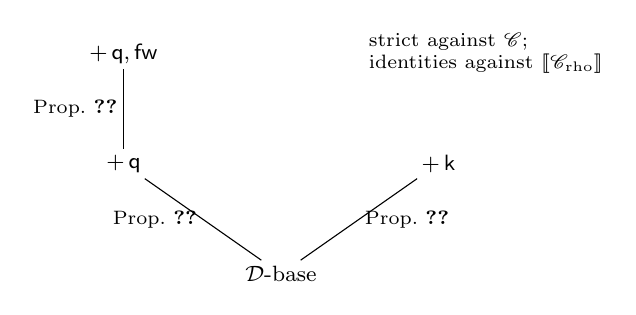
\begin{tikzpicture}[scale=1.0, every node/.style={font=\footnotesize, inner sep=2pt}]
\node (o0)  at (0,0)       {$\Obs$-base};
\node (oq)  at (-2.0,1.4)  {$+\,\qq$};
\node (ok)  at (2.0,1.4)   {$+\,\kk$};
\node (oqf) at (-2.0,2.8)  {$+\,\qq,\fw$};
\draw (o0) -- node[left, font=\scriptsize] {Prop.~\ref{prop:collapse}} (oq);
\draw (o0) -- node[right, font=\scriptsize] {Prop.~\ref{prop:collapse}} (ok);
\draw (oq) -- node[left, font=\scriptsize] {Prop.~\ref{prop:fwq}} (oqf);
\node[font=\scriptsize, align=left] at (2.6,2.8)
  {strict against $\Ctx$;\\ identities against $\enc{\Ctx_{\mathrm{rho}}}$};
\end{tikzpicture}
\caption{The observational lattice over the same base. Each edge is strict
against arbitrary combinator contexts and an identity against encoded ones,
so this entire figure collapses to its bottom point in
Figure~\ref{fig:exprlattice}. The $\fw$ edge sits above the $\qq$ node rather
than over the base, since $\fw$ is redundant when $\qq$ is absent and
essential when it is present. No edge is drawn from the base to $\fw$ alone:
by Proposition~\ref{prop:fwq} there is none.}
\label{fig:obslattice}
\end{figure}

So $\qq$ occupies the same point as $\mm$ on the expressiveness ordering and
a strictly different one on the observational ordering. These are two
orderings on the same subsets and they do not coincide ---
Figures~\ref{fig:exprlattice} and~\ref{fig:obslattice} --- which is the
structural difference from Yoshida's setting: she has $\mathsf{new}$, so a
constructed name can be hidden and the two orderings agree. Several of her
separation arguments turn on exactly that hiding and do not transfer; they
want redoing rather than citing, and we have not done so here.

\subsection{Summary}

\begin{figure}[t]
\centering
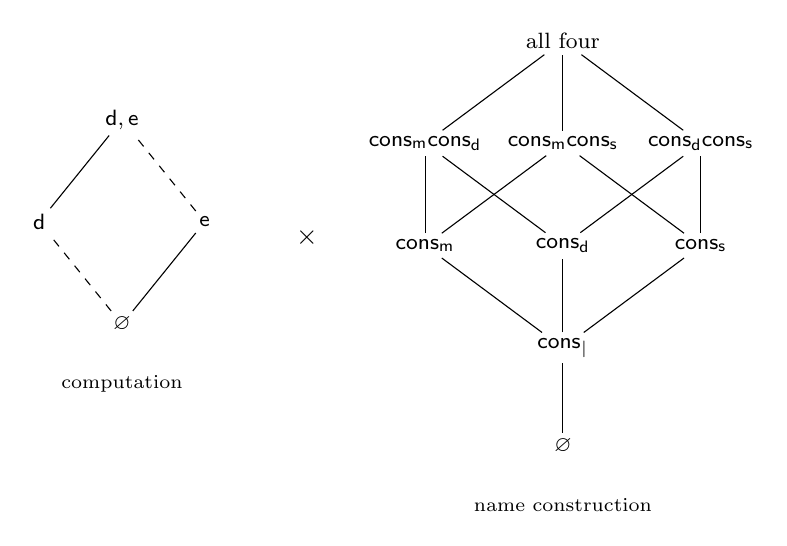
\begin{tikzpicture}[scale=1.0, every node/.style={font=\footnotesize, inner sep=2pt}]
% --- computation axis ---
\node (a0)  at (0,0.9)      {$\varnothing$};
\node (ad)  at (-1.05,2.2) {$\dd$};
\node (ae)  at (1.05,2.2)  {$\ev$};
\node (ade) at (0,3.5)     {$\dd,\ev$};
\draw[dashed] (a0) -- (ad);
\draw         (a0) -- (ae);
\draw         (ad) -- (ade);
\draw[dashed] (ae) -- (ade);
\node[font=\scriptsize] at (0,0.15) {computation};
\node[font=\normalsize] at (2.35,2.0) {$\times$};
% --- constructor axis ---
\begin{scope}[xshift=5.6cm]
  \node (b0)  at (0,-0.65)   {$\varnothing$};
  \node (bp)  at (0,0.6)     {$\cons_{\mid}$};
  \node (bm)  at (-1.75,1.9) {$\cons_{\mm}$};
  \node (bd)  at (0,1.9)     {$\cons_{\dd}$};
  \node (bs)  at (1.75,1.9)  {$\cons_{\sy}$};
  \node (bmd) at (-1.75,3.2) {$\cons_{\mm}\cons_{\dd}$};
  \node (bms) at (0,3.2)     {$\cons_{\mm}\cons_{\sy}$};
  \node (bds) at (1.75,3.2)  {$\cons_{\dd}\cons_{\sy}$};
  \node (ball) at (0,4.5)    {all four};
  \draw (b0) -- (bp);
  \draw (bp) -- (bm); \draw (bp) -- (bd); \draw (bp) -- (bs);
  \draw (bm) -- (bmd); \draw (bm) -- (bms);
  \draw (bd) -- (bmd); \draw (bd) -- (bds);
  \draw (bs) -- (bms); \draw (bs) -- (bds);
  \draw (bmd) -- (ball); \draw (bms) -- (ball); \draw (bds) -- (ball);
  \node[font=\scriptsize] at (0,-1.4) {name construction};
\end{scope}
\end{tikzpicture}
\caption{The expressive lattice, as a product of two independent axes over the
base of $\mm$ and the routers. Nodes above $\cons_{\mid}$ carry it
implicitly. Solid edges are strict by Propositions~\ref{prop:consedges}
and~\ref{prop:sn} and Corollary~\ref{cor:boolean}; dashed edges are
Conjecture~\ref{conj:dup} and the open question of whether duplication alone
adds anything in the absence of $\ev$. The atoms $\qq$, $\kk$ and $\fw$ do
not appear: on this ordering $\qq$ sits at the point of $\mm$, and $\kk$ and
$\fw$ are derivable from the remaining routers
(Propositions~\ref{prop:fwq} and~\ref{prop:collapse}).}
\label{fig:exprlattice}
\end{figure}

\begin{center}
\begin{tabular}{@{}lll@{}}
\toprule
edge & status & by\\
\midrule
$\cons_{\mid}$ over no constructors & strict & Prop.~\ref{prop:consedges}\\
$\cons_{\mm}$, $\cons_{\dd}$, $\cons_{\sy}$, pairwise & strict &
  Cor.~\ref{cor:boolean}\\
$\ev$ over no $\ev$ & strict & Prop.~\ref{prop:sn}\\
$\dd$ over no $\dd$ & conjectured strict & Conj.~\ref{conj:dup}\\
$\fw$, given $\qq$ & strict & Prop.~\ref{prop:fwq}\\
$\fw$, without $\qq$ & collapses, given $\dd,\kk$ & Prop.~\ref{prop:fwq}\\
$\qq$ over $\mm$ & collapses for encoded observers & Prop.~\ref{prop:collapse}\\
$\kk$ over $\sy$ & collapses for encoded observers & Prop.~\ref{prop:collapse}\\
$\bl$, $\br$, $\sy$, pairwise & open &\\
\bottomrule
\end{tabular}
\end{center}

The last row is the gap. Yoshida separates her binders from one another, and
the corresponding question here is genuinely open rather than inherited,
because her arguments use hiding and ours cannot.

\section{An alternative presentation: constructors only}
\label{sec:altpres}

The calculus of \S\ref{sec:comb} has three kinds of atom doing three jobs:
routers ($\dd,\kk,\fw,\bl,\br,\sy$), which move names; a destructor ($\ev$),
which opens one; and value-bearing atoms ($\mm$, $\qq$, $\cons$). The third
group is not three things but one.

\begin{remark}
Read a constructor as a dataflow node: $\cons_{A}(a_{1},\dots,a_{n},c)$ says
that when names are available at $a_{1},\dots,a_{n}$, the name $A$ of them is
available at $c$. Then $\mm(c,v)$ is the nullary case --- the name $v$ is
available at $c$, unconditionally --- and $\qq(c,v)$ is the nullary case in a
quiet variant. On this reading neither $\mm$ nor $\qq$ is primitive: the
calculus consists of routers, one destructor, and a constructor family whose
arity-zero members are the messages.
\end{remark}

Two things recommend this presentation. It is uniform: every atom takes names
and every rule is either routing, opening, or building, with no atom indexed
by a process. And it makes Remark~\ref{rem:loudquiet} a question about the
family rather than about two special atoms --- whether a constructor's output
is loud or quiet is a single design parameter, and $\mm$ versus $\qq$ is its
nullary instance.

Two things count against it, and we record them rather than settle them.
Barbs, or their context-labelled counterpart, need a notion of message; if
messages are nullary constructors then observation must be defined on the
constructor family, which is a mild complication but changes what
Lemma~\ref{lem:usage} has to say. And a calculus closed under its own
constructions would need one member per atom shape, including members for the
constructors themselves, since a constructed name may quote a term containing
one; the four of Proposition~\ref{prop:four} suffice for the image of the
translation but not for that closure. The context-indexed atom of
Remark~\ref{rem:ctxindexed} sidesteps the regress at a conceptual price we
judge too high. Which to prefer is a genuine choice, and the results of this
note hold either way.

\section{Corrigenda to \cite{rhocomb}}
\label{sec:corrigenda}

Restricted to what bears on the rho calculus; the material specific to the
$\pi$-calculus route is out of scope here.

\begin{enumerate}[leftmargin=1.6em]
\item \textbf{The drop and the guard are conflated.} The published grammar
writes both as $\mathsf{*}$ and lists the guard under the process
production, which makes every running process a redex
(Proposition~\ref{prop:defect}). They must be separate constructors. The
equation $\mathsf{*}(\quo{P}) = P$ may then be kept or omitted
(\S\ref{sec:two}); it is not the source of the unsoundness.

\item \textbf{The binders produce messages rather than forwarders} in some
statements of the rules, which collapses them into $\mathsf{forward}$; see
Remark~\ref{rem:departures}, which also records the arity slips in $\fw$ and
in the constructors' delivery channel.

\item \textbf{No rho-to-combinator translation is given.} The outline
promises that the encoding of a source calculus into the combinators
composes with an encoding into the rho calculus, but the translation defined
in the body has Yoshida terms as its domain. \S\ref{sec:translation} supplies
the missing map, and \S\ref{sec:lattice} shows that no such map exists
without a name constructor.

\item \textbf{No prefix-elimination lemma.} The draft states two theorems and
proves no lemmas. The prefixed form $\mathsf{for}(x \leftarrow p)C$ is never
given a semantics in the combinator calculus, so the correctness of
elimination is neither stated nor proved. Lemmas~\ref{lem:gate}
to~\ref{lem:release} are the analogue here.

\item \textbf{$\nequiv$ is undefined for the combinators} yet is used in the
side condition on observation.

\item \textbf{Name sizes.} Constructed names quote the subterm they must be
fresh for, making the output quadratic before other costs
(Remark~\ref{rem:namesize}).

\item \textbf{Typing slips.} $x^{l} := \quo{\bl(x,\mm(x,\drp{x}))}$ puts a
process in the second argument of $\bl$, which takes names. The derivation
following the definition of the replication server carries a spurious extra
copy of $\mm(x,\quo{(D \mid P)})$ on its third line; the calculation is
otherwise correct. Polarity annotations appear inside quoted terms, and
several where-clauses construct names mentioning a bound variable, which is a
metavariable rather than a name of the calculus.
\end{enumerate}

\section{Open questions}

\begin{enumerate}[leftmargin=1.6em]
\item \textbf{Minimal labels.} Theorem~\ref{thm:fullabs} uses enabling
contexts. The minimal-label form, via relative pushouts taken in the image of
the translation, is the discipline of \cite{BIHOL}; the forward half descends
for free and the backward half is what is owed.

\item \textbf{Loud and quiet constructors} (Remark~\ref{rem:loudquiet}).
Should every constructor have a quiet variant, and does the quiet calculus
admit a sharper form of Proposition~\ref{prop:forced}?

\item \textbf{Name growth.} With the constructors, names are no longer subterms of the
program: they grow at runtime. The consequences for the decidability of
$\nequiv$ in practice, and for cost accounting, want examining.

\item \textbf{The open edges of the lattice} (\S\ref{sec:lattice}):
Conjecture~\ref{conj:dup}, and the mutual independence of $\bl$, $\br$ and
$\sy$ without recourse to hiding.

\item \textbf{Is four minimal?} Proposition~\ref{prop:four} gives an upper
bound for the uniform translation, and Remark~\ref{rem:optnotfree} shows the
count is translation-relative. Is there a translation needing fewer, is
$\cons_{\mid}$ alone enough for some reformulation, and does reflection make
any of Yoshida's six routers redundant?
\end{enumerate}

\begin{thebibliography}{99}

\bibitem{BIHOL} C.\,B. Wells, M. Stay and L.\,G. Meredith.
\emph{Behavior in higher-order languages: admissible observers, relative
pushouts, and the encoding of extended theories.}
In preparation, F1R3FLY.io, 2026.

\bibitem{Lybech22} S. Lybech.
\emph{Encodability and separation for a reflective higher-order calculus.}
EXPRESS/SOS 2022, EPTCS 368, 95--112.

\bibitem{MeredithRadestock05} L.\,G. Meredith and M. Radestock.
\emph{A reflective higher-order calculus.}
Electronic Notes in Theoretical Computer Science 141(5):49--67, 2005.

\bibitem{nowns} L.\,G. Meredith.
\emph{Namespaces without a name server: freshness by communication, and a
fully abstract encoding of the $\pi$-calculus in the rho calculus.}
F1R3FLY.io, 2026.

\bibitem{rhocomb} L.\,G. Meredith and M. Stay.
\emph{Name-free combinators for concurrency.}
Working draft, \texttt{rho4u}.

\bibitem{Yoshida02} N. Yoshida.
\emph{Minimality and separation results on asynchronous mobile processes:
representability theorems by concurrent combinators.}
Theoretical Computer Science 274(1--2):231--276, 2002.

\end{thebibliography}

\end{document}
